% figures/new/fig_participation_saving.tex -- Appendix Figure C3 (fig:participation_saving), written by W3. Self-contained float
% (BLUEPRINT 2.7 exhibits; Override O6). Input from appendix/C_reforms.tex.
% Built only from printed cells of tables/welfare_age_dependence_mvpfv5.tex. Each point is (Direct, participation change at 62-64)
% in panel A and (Direct, participation change at 65-69) in panel B; Direct in percent of baseline retirement benefits, participation in pp.
%   AN1 :108  Direct -6.13   62-64  0.38   65-69 0.60
%   AN2 :109  Direct -11.82  62-64 -0.04   65-69 1.98
%   AN3 :110  Direct -16.75  62-64 -0.43   65-69 3.27
%   AD1 :112  Direct -2.46   62-64  0.15   65-69 0.74
%   AD2 :113  Direct -2.87   62-64  0.18   65-69 0.57
%   AD3 :114  Direct -4.22   62-64 -0.36   65-69 1.20
%   AD4 :115  Direct -4.56   62-64 -0.49   65-69 1.37
%   AD5 :116  Direct -5.05   62-64 -0.97   65-69 1.39
%   AL1 :118  Direct -0.74   62-64  0.24   65-69 0.22
%   AL2 :119  Direct -2.81   62-64  0.05   65-69 0.61
%   AL3 :120  Direct -4.74   62-64 -0.31   65-69 1.21
%   AL4 :121  Direct -5.54   62-64 -0.93   65-69 1.42
%   AL5 :122  Direct -7.02   62-64 -1.15   65-69 2.01
%   AL6 :123  Direct -7.72   62-64 -1.46   65-69 2.61
%   AL7 :124  Direct -8.21   62-64 -2.90   65-69 2.50
%   AL8 :125  Direct -8.22   62-64 -3.30   65-69 2.42
%   AL9 :126  Direct -8.45   62-64 -3.49   65-69 2.26
% House style: grid, legend below; FROT palette from preamble.tex. Marker by family: AN squares, AD circles, AL triangles.
\begin{figure}[!t]
\centering
\caption{Participation Changes at Ages 62--64 and 65--69 against the Direct Fiscal Effect, Claiming-Schedule Reforms}
\label{fig:participation_saving}
\vspace{6pt}
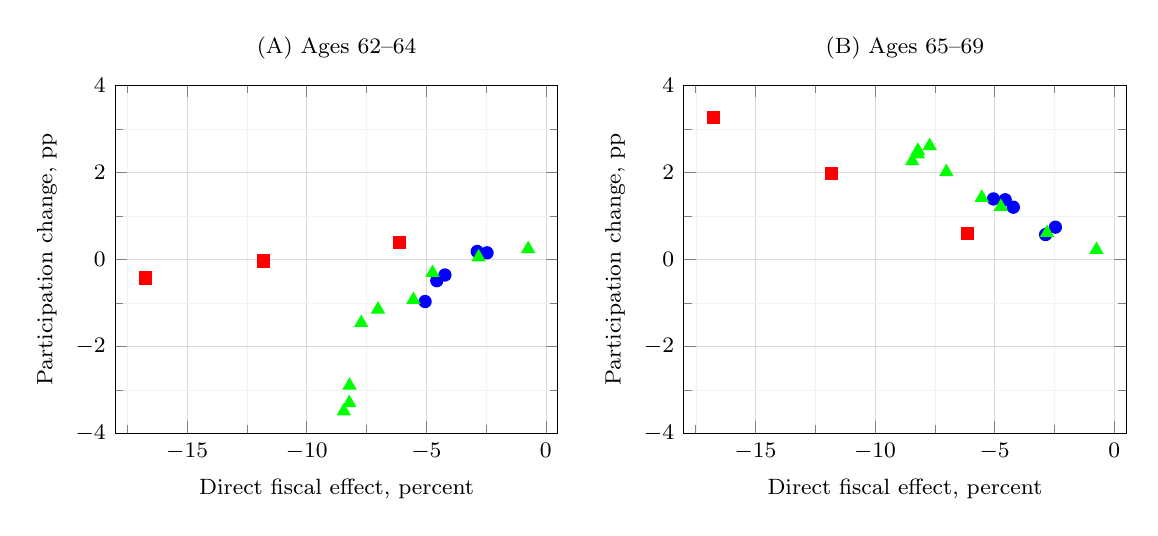
\begin{tikzpicture}
\begin{axis}[%
name=panelA,
width=7.2cm,
height=6cm,
title={(A) Ages 62--64},
title style={font=\footnotesize},
xlabel={Direct fiscal effect, percent},
ylabel={Participation change, pp},
xmin=-18, xmax=0.5,
ymin=-4, ymax=4,
grid=both,
grid style={line width=0.2pt, draw=gray!30},
minor grid style={line width=0.1pt, draw=gray!10},
minor tick num=1,
axis background/.style={fill=white},
tick label style={font=\footnotesize},
label style={font=\footnotesize},
legend to name=legpartsave,
legend columns=3,
legend style={draw=white!15!black, font=\scriptsize, /tikz/every even column/.append style={column sep=0.6em}},
legend cell align=left
]
\addplot [only marks, color=red, mark=square*, mark size=2.2pt] coordinates {(-6.13,0.38) (-11.82,-0.04) (-16.75,-0.43)};          % src: tables/welfare_age_dependence_mvpfv5.tex:108-110
\addlegendentry{Higher NRA (AN1--AN3)}
\addplot [only marks, color=blue, mark=*, mark size=2.2pt] coordinates {(-2.46,0.15) (-2.87,0.18) (-4.22,-0.36) (-4.56,-0.49) (-5.05,-0.97)};   % src: tables/welfare_age_dependence_mvpfv5.tex:112-116
\addlegendentry{Higher DRC (AD1--AD5)}
\addplot [only marks, color=green, mark=triangle*, mark size=2.6pt] coordinates {(-0.74,0.24) (-2.81,0.05) (-4.74,-0.31) (-5.54,-0.93) (-7.02,-1.15) (-7.72,-1.46) (-8.21,-2.90) (-8.22,-3.30) (-8.45,-3.49)};   % src: tables/welfare_age_dependence_mvpfv5.tex:118-126
\addlegendentry{Symmetric adjustment (AL1--AL9)}
\end{axis}
\begin{axis}[%
at={(panelA.east)}, anchor=west, xshift=1.6cm,
width=7.2cm,
height=6cm,
title={(B) Ages 65--69},
title style={font=\footnotesize},
xlabel={Direct fiscal effect, percent},
ylabel={Participation change, pp},
xmin=-18, xmax=0.5,
ymin=-4, ymax=4,
grid=both,
grid style={line width=0.2pt, draw=gray!30},
minor grid style={line width=0.1pt, draw=gray!10},
minor tick num=1,
axis background/.style={fill=white},
tick label style={font=\footnotesize},
label style={font=\footnotesize}
]
\addplot [only marks, color=red, mark=square*, mark size=2.2pt] coordinates {(-6.13,0.60) (-11.82,1.98) (-16.75,3.27)};          % src: tables/welfare_age_dependence_mvpfv5.tex:108-110
\addplot [only marks, color=blue, mark=*, mark size=2.2pt] coordinates {(-2.46,0.74) (-2.87,0.57) (-4.22,1.20) (-4.56,1.37) (-5.05,1.39)};   % src: tables/welfare_age_dependence_mvpfv5.tex:112-116
\addplot [only marks, color=green, mark=triangle*, mark size=2.6pt] coordinates {(-0.74,0.22) (-2.81,0.61) (-4.74,1.21) (-5.54,1.42) (-7.02,2.01) (-7.72,2.61) (-8.21,2.50) (-8.22,2.42) (-8.45,2.26)};   % src: tables/welfare_age_dependence_mvpfv5.tex:118-126
\end{axis}
\end{tikzpicture}

\vspace{2pt}
\pgfplotslegendfromname{legpartsave}

\begin{minipage}{0.92\textwidth}
\vspace{4pt}
\scriptsize
\textit{Notes:} Each marker is one row of \autoref{tab:claiming}. The horizontal axis is the Direct column, the change in the net present value of retirement benefits paid to the cohort as a percentage of its baseline value; the vertical axis is the change in labor force participation in percentage points (pp) at ages 62--64 (panel A) and 65--69 (panel B). Squares: a higher normal retirement age (AN1--AN3); circles: a higher delayed retirement credit (AD1--AD5); triangles: equal early-claiming reductions and delayed credits of $\pm7$ to $\pm15$ percent per year (AL1--AL9). Source: authors' simulations of the estimated model.
% src: tables/welfare_age_dependence_mvpfv5.tex:108-126
\end{minipage}
\end{figure}
